\section{Basics}
     \begin{multicols}{2}
        DBS = DBMS + (n*)DB
        \begin{description}
        \setlength{\itemsep}{0pt}    
            \item[DBS] Datenbanksystem
            \item[DBMS] Datenbankmanagementsystem
            \item[DB] Datenbasis
        \end{description}
%         \includegraphics[page=13,trim=20 40 20 140,clip=true,width=0.5\textwidth]{images/einfuehrung.pdf}
     \end{multicols}
    \subsection {DBMS}
    \begin{multicols}{2}
        \subsubsection{Eigenschaften}
            \begin{itemize}
            \setlength{\itemsep}{0pt}
              \item Verwaltet zentrale Datenbasis (Datenbank)
              \item Anwendungen greifen via DBMS auf die Daten zu
              \item Die Daten sind strukturiert und die Struktur ist im Datenkatalog beschrieben
              \item Client-Server Struktur
              \item Sichert Datenintegrität
              \item Stellt Datenpflege, Datenschutz und Datensicherheit sicher
            \end{itemize}
        \subsubsection{Anforderungen}
           \begin{itemize}
           \setlength{\itemsep}{0pt}
             \item Redundanzfreiheit
             \item Datenintegrität (Kosistenz, Sicherheit, Schutz)
           \end{itemize}
        \subsubsection{Funktionen}
            \begin{itemize}
            \setlength{\itemsep}{0pt}  
              \item Transaktionen
              \item Synchronisation paralleler Zugriffe (Mehrnutzerbetrieb)
              \item Sicherheit: Authentifizierung, Autorisierung
              \item Backup und Recovery
              \item Abfragesprache, Schnittstellen
            \end{itemize}
        \subsubsection{Modelle}
            \begin{itemize}
            \setlength{\itemsep}{0pt}    
                \item Hierarchisches DBM (XML)
                \item Netzwerk-DBM
                \item Relationales-DBM (SQL)
                \item Postrelationale-DBM (OODB)
            \end{itemize}
    \end{multicols}            
    \begin{multicols}{2}            
        \subsection{3-Ebenen-Modell}
            \includegraphics[page=22,trim=20 40 20 100,clip=true,width=0.4\textwidth]{images/einfuehrung.pdf}
        \subsection{Entwurfsprozess}
            \includegraphics[page=26,trim=20 20 20 85,clip=true,width=0.4\textwidth]{images/einfuehrung.pdf}
    \end{multicols}        